% =====================================================================
%  Chapitre 2 -- L'operation de convolution
%  Partie c : noyaux classiques, effets, convolution 1D, cout de calcul,
%             quiz, a retenir, TP1 / TP2
% =====================================================================

\begin{frame}{Les noyaux classiques : convoluer avant d'apprendre}
\begin{columns}[t]
\begin{column}{0.50\textwidth}
\begin{itemize}
  \item Le traitement d'image utilise la convolution depuis les années 1960,
  bien avant les CNN.
  \item Les ingénieurs écrivaient les noyaux \textbf{à la main}, en
  choisissant chaque coefficient selon l'effet voulu.
  \item Un noyau est donc une \textbf{petite matrice de coefficients} que
  l'on fait glisser sur l'image.
  \item Ces noyaux sont toujours utiles aujourd'hui :
  \begin{itemize}
    \item pour nettoyer une image avant de la donner au réseau ;
    \item pour comprendre, par contraste, ce qu'un CNN \emph{apprend} lui-même.
  \end{itemize}
\end{itemize}

\end{column}
\begin{column}{0.47\textwidth}
\begin{figbox}
\centering
\end{figbox}
\end{column}
\end{columns}
% [fix] figure sortie
% [fix] bloc deplace
\end{frame}
\begin{frame}{Les noyaux classiques : convoluer avant … (suite)}
\begin{kbox}[L'idée à garder]
Un noyau classique encode une action locale : moyenne, écart entre voisins,
variation dans une direction. Le CNN ne fait rien d'autre --- il choisit ces
coefficients par apprentissage au lieu de les écrire.
\end{kbox}
\end{frame}

\begin{frame}{Les noyaux classiques : convoluer avant d'apprendre --- la figure}\begin{center}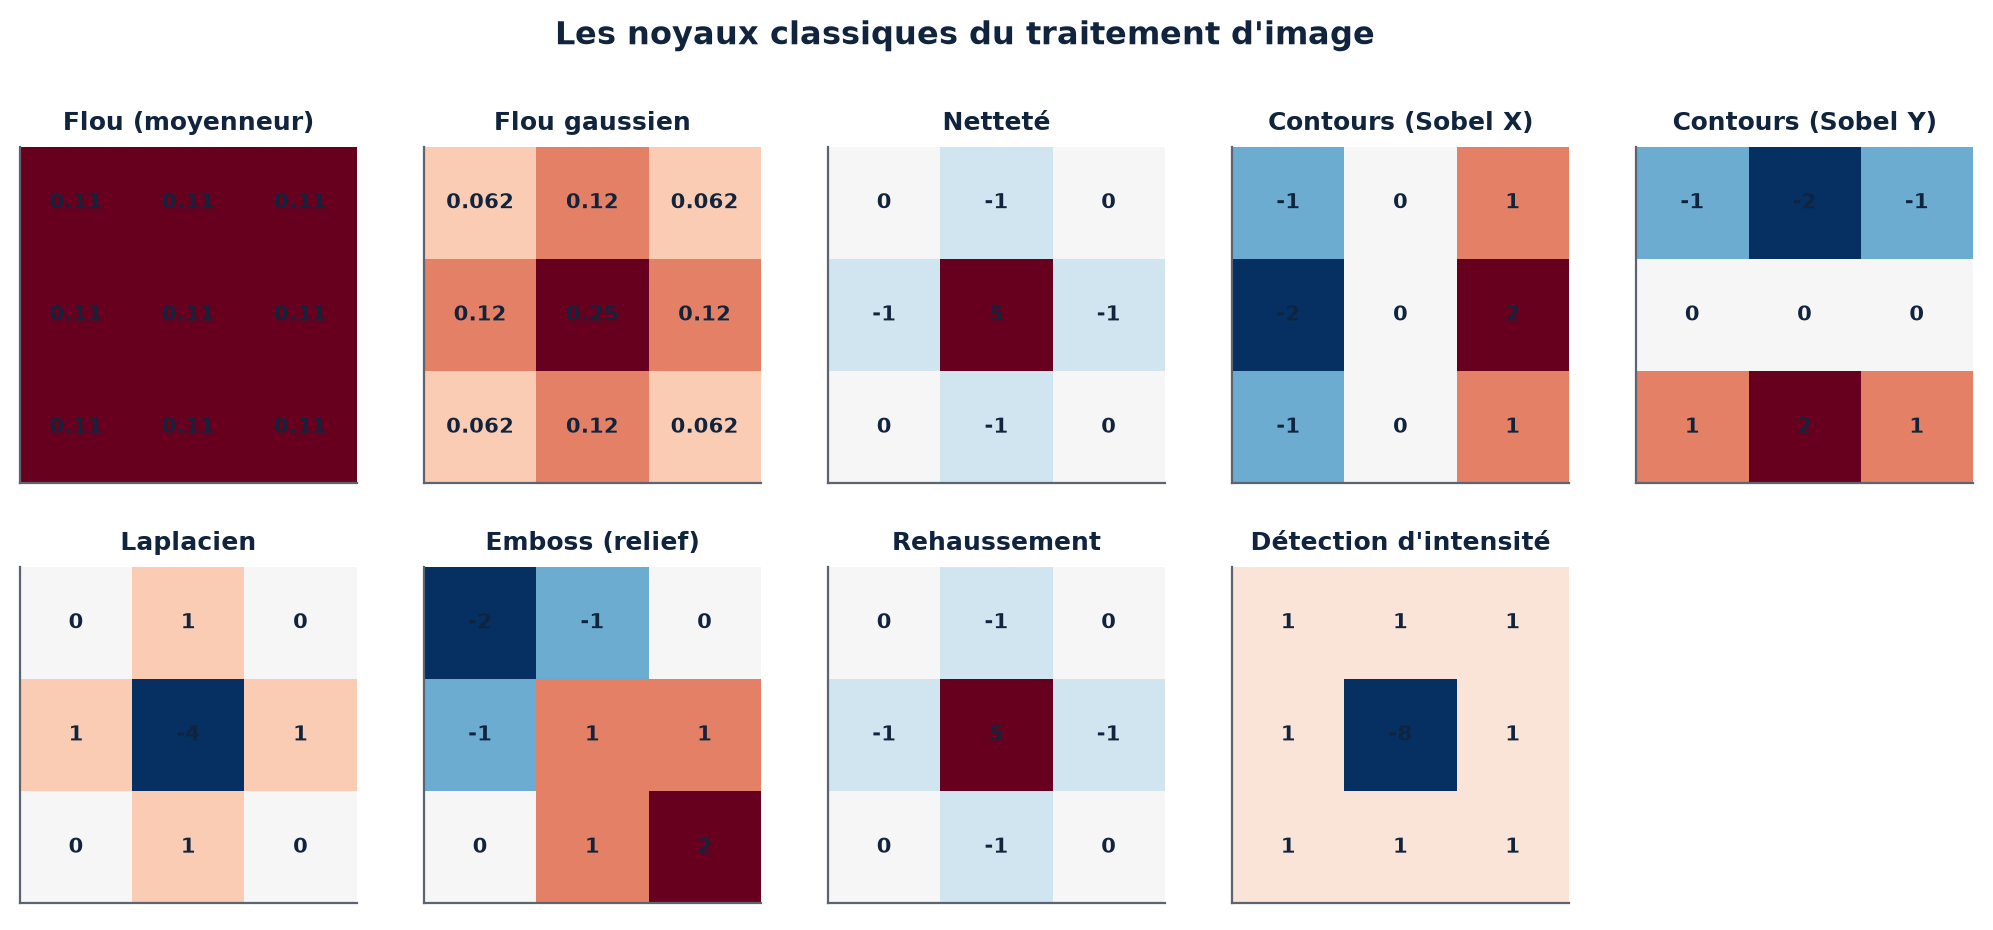
\includegraphics[width=.92\textwidth]{g03_noyaux_classiques.png}\end{center}\end{frame}

\begin{frame}{Les matrices exactes des noyaux (1/2)}
\begin{center}
{\scriptsize
\setlength{\arraycolsep}{4pt}
\begin{tabular}{@{}l c l c@{}}
\toprule
\textbf{Noyau} & \textbf{Matrice} & \textbf{Noyau} & \textbf{Matrice} \\
\midrule
\addlinespace
Flou\newline (moyenneur) &
$\dfrac{1}{9}\begin{smallmatrix}1&1&1\\1&1&1\\1&1&1\end{smallmatrix}$ &
Flou\newline gaussien &
$\dfrac{1}{16}\begin{smallmatrix}1&2&1\\2&4&2\\1&2&1\end{smallmatrix}$ \\
\addlinespace
Netteté &
$\begin{smallmatrix}0&-1&0\\-1&5&-1\\0&-1&0\end{smallmatrix}$ &
Laplacien &
$\begin{smallmatrix}0&1&0\\1&-4&1\\0&1&0\end{smallmatrix}$ \\
\addlinespace
\bottomrule
\end{tabular}
}
\end{center}
\vspace{1mm}
\begin{columns}[t]
\begin{column}{0.48\textwidth}
\begin{itemize}
  \item \textbf{Flou moyenneur} : les $9$ coefficients valent $1/9$, leur
  somme vaut $1$ $\Rightarrow$ la luminosité moyenne est conservée.
  \item \textbf{Flou gaussien} : les poids décroissent avec la distance,
  le centre pèse $4/16$ ; le résultat est plus doux, sans « carré ».
\end{itemize}
\end{column}
\begin{column}{0.48\textwidth}
\begin{itemize}
  \item \textbf{Netteté} : le centre est accentué ($5$) et les quatre
  voisins directs sont soustraits ($-1$) : somme $= 1$.
  \item \textbf{Laplacien} : la somme des coefficients vaut $0$ : un
  voisinage \emph{uniforme} donne toujours $0$.
\end{itemize}
\end{column}
\end{columns}
\end{frame}

\begin{frame}{Les matrices exactes des noyaux (2/2)}
\begin{center}
{\scriptsize
\setlength{\arraycolsep}{4pt}
\begin{tabular}{@{}l c l c@{}}
\toprule
\textbf{Noyau} & \textbf{Matrice} & \textbf{Noyau} & \textbf{Matrice} \\
\midrule
\addlinespace
Contours\newline (Sobel X) &
$\begin{smallmatrix}-1&0&1\\-2&0&2\\-1&0&1\end{smallmatrix}$ &
Contours\newline (Sobel Y) &
$\begin{smallmatrix}-1&-2&-1\\0&0&0\\1&2&1\end{smallmatrix}$ \\
\addlinespace
Emboss\newline (relief) &
$\begin{smallmatrix}-2&-1&0\\-1&1&1\\0&1&2\end{smallmatrix}$ &
Détection\newline d'intensité &
$\begin{smallmatrix}1&1&1\\1&-8&1\\1&1&1\end{smallmatrix}$ \\
\addlinespace
\bottomrule
\end{tabular}
}
\end{center}
\vspace{1mm}
\begin{columns}[t]
\begin{column}{0.48\textwidth}
\begin{itemize}
  \item \textbf{Sobel X} : différence gauche/droite $\Rightarrow$ il répond
  aux \textbf{contours verticaux}.
  \item \textbf{Sobel Y} : différence haut/bas $\Rightarrow$ il répond aux
  \textbf{contours horizontaux}.
\end{itemize}
\begin{ebox}[Pourquoi ces coefficients $2$ au centre ?]
$1,2,1$ est le lissage d'une dérivée : on moyenne selon l'axe
\emph{perpendiculaire} au contour, ce qui rend la détection moins sensible au bruit.
\end{ebox}
\end{column}
\begin{column}{0.48\textwidth}
\begin{itemize}
  \item \textbf{Emboss} : noyau antisymétrique en diagonale ; somme $= 1$
  (l'image reste lisible), mais les bords prennent un aspect de gravure.
  \item \textbf{Détection d'intensité} : un pixel très différent de ses
  $8$ voisins ressort violemment (somme $= 0$).
\end{itemize}

\end{column}
\end{columns}
% [fix] bloc deplace
\end{frame}
\begin{frame}{Les matrices exactes des noyaux (2/2) (suite)}
\begin{wbox}[Règle de lecture]
La \textbf{somme des coefficients} fixe le comportement sur une zone
uniforme : égale à $1$ $\Rightarrow$ l'image est conservée ; égale à $0$
$\Rightarrow$ les zones uniformes deviennent noires.
\end{wbox}
\end{frame}

\begin{frame}{Effets comparés sur une image réelle}
\begin{columns}[t]
\begin{column}{0.62\textwidth}
\begin{figbox}
\centering
\end{figbox}
\end{column}
\begin{column}{0.36\textwidth}
\begin{itemize}
  \item \textbf{Originale} : référence.
  \item \textbf{Flou} : les détails fins disparaissent, les bords deviennent
  progressifs.
  \item \textbf{Gaussien} : lissage plus régulier, sans direction privilégiée.
  \item \textbf{Netteté} : les bords sont marqués, mais le bruit est
  \emph{amplifié}.
  \item \textbf{Contours Sobel} : le contenu disparaît, il ne reste que les
  zones de forte variation.
  \item \textbf{Contours Laplacien} : variante isotrope, plus fine mais très
  sensible au bruit.
\end{itemize}

\end{column}
\end{columns}
% [fix] figure sortie
% [fix] bloc deplace
\end{frame}
\begin{frame}{Effets comparés sur une image réelle (suite)}
\begin{kbox}[Lecture]
Ces six images sortent de la \emph{même} opération : seule la matrice des
coefficients change.
\end{kbox}
\end{frame}

\begin{frame}{Effets comparés sur une image réelle --- la figure}\begin{center}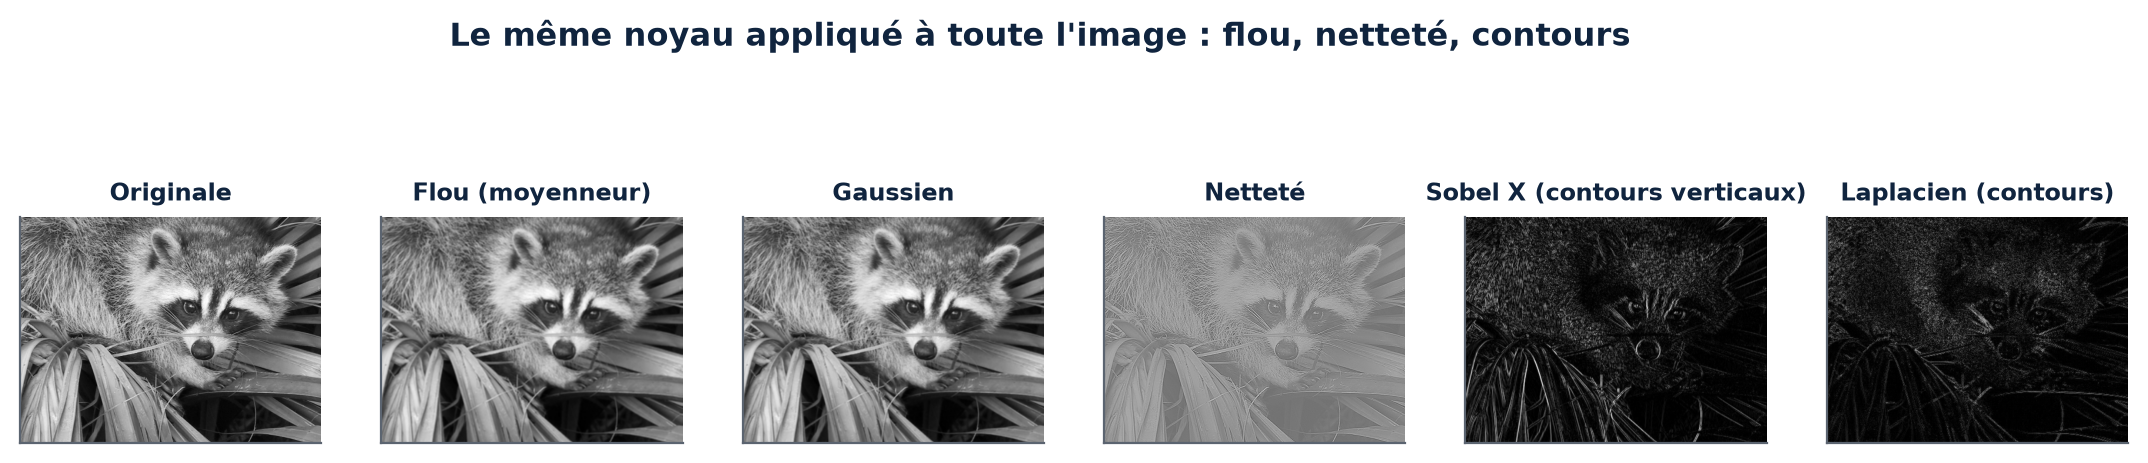
\includegraphics[width=.92\textwidth]{g04_effets_noyaux.png}\end{center}\end{frame}

\begin{frame}{Ce que fait chaque famille de noyaux}
\begin{center}
\begin{tabular}{@{}p{3.4cm} p{5.4cm} p{4.4cm}@{}}
\toprule
\textbf{Famille} & \textbf{Action} & \textbf{Somme des coefficients} \\
\midrule
Flou (moyenneur, gaussien) & moyenne pondérée du voisinage : basse fréquence &
égale à $1$ \\
Netteté, rehaussement & amplifie le centre, soustrait le voisinage : haute
fréquence & égale à $1$ \\
Contours (Sobel, Prewitt) & dérivée dans une direction : gradient &
égale à $0$ \\
Laplacien, intensité & dérivée seconde : variations brusques & égale à $0$ \\
Emboss (relief) & gradient orienté, rendu de relief & égale à $1$ \\
\bottomrule
\end{tabular}
\end{center}
\vspace{1mm}
\begin{wbox}[Deux précautions]
\begin{itemize}
  \item Un noyau de somme nulle peut produire des valeurs \textbf{négatives} :
  il faut décider d'une convention d'affichage ou de valeur absolue.
  \item Après convolution, l'échelle change : penser à normaliser (par exemple
  ramener sur $[0, 255]$) avant d'afficher.
\end{itemize}
\end{wbox}
\end{frame}

\begin{frame}{Le noyau moyen : pourquoi cela floute}
\begin{columns}[t]
\begin{column}{0.48\textwidth}
\begin{itemize}
  \item Chaque pixel de sortie remplace le pixel d'entrée par la
  \textbf{moyenne} de son voisinage $3 \times 3$.
  \item Un pixel isolé, très clair ou très sombre, est « noyé » dans ses
  voisins : c'est exactement la disparition des détails fins.
  \item Le flou moyenneur est donc un \textbf{filtre passe-bas} :
  il garde les structures lentes, supprime les variations rapides.
  \item Plus le noyau est grand, plus l'effet est fort
  ($3\times3$, $5\times5$, \dots).
\end{itemize}
\end{column}
\begin{column}{0.48\textwidth}
\begin{ebox}[Vérification sur un cas simple]
Prenons trois pixels alignés : $10$, $200$, $12$.
La moyenne des trois vaut $(10 + 200 + 12)/3 = 74$.

\medskip
Le pic $200$ devient $74$ : l'écart avec ses voisins passe de $188$ à
environ $60$. Le détail est bien atténué.
\end{ebox}
\begin{wbox}[Le revers]
Flouter ne crée aucune information : cela en \textbf{détruit}. Un réseau
entraîné sur des images trop floues apprend sur des données appauvries.
\end{wbox}
\end{column}
\end{columns}
\end{frame}

\begin{frame}{La convolution 1D : même opération, une seule direction}
\begin{columns}[t]
\begin{column}{0.56\textwidth}
\begin{figbox}
\centering
\end{figbox}
\end{column}
\begin{column}{0.42\textwidth}
\begin{itemize}
  \item Un signal est une \textbf{suite de valeurs indexées par le temps} :
  $x[0], x[1], \dots, x[N-1]$.
  \item Le noyau devient un \textbf{vecteur} de longueur $K$.
  \item La convolution parcourt le signal de gauche à droite, exactement
  comme le noyau $2$D parcourt l'image.
  \item Toute la machinerie des CNN s'applique : localité, partage de poids,
  cartes de sortie, empilement de couches.
\end{itemize}

\end{column}
\end{columns}
% [fix] figure sortie
% [fix] bloc deplace
\end{frame}
\begin{frame}{La convolution 1D : même opération, une … (suite)}
\begin{kbox}[Formule]
\[
y[n] = \sum_{k=0}^{K-1} x[n+k]\,h[k]
\]
\end{kbox}
\end{frame}

\begin{frame}{La convolution 1D : même opération, une seule direction --- la figure}\begin{center}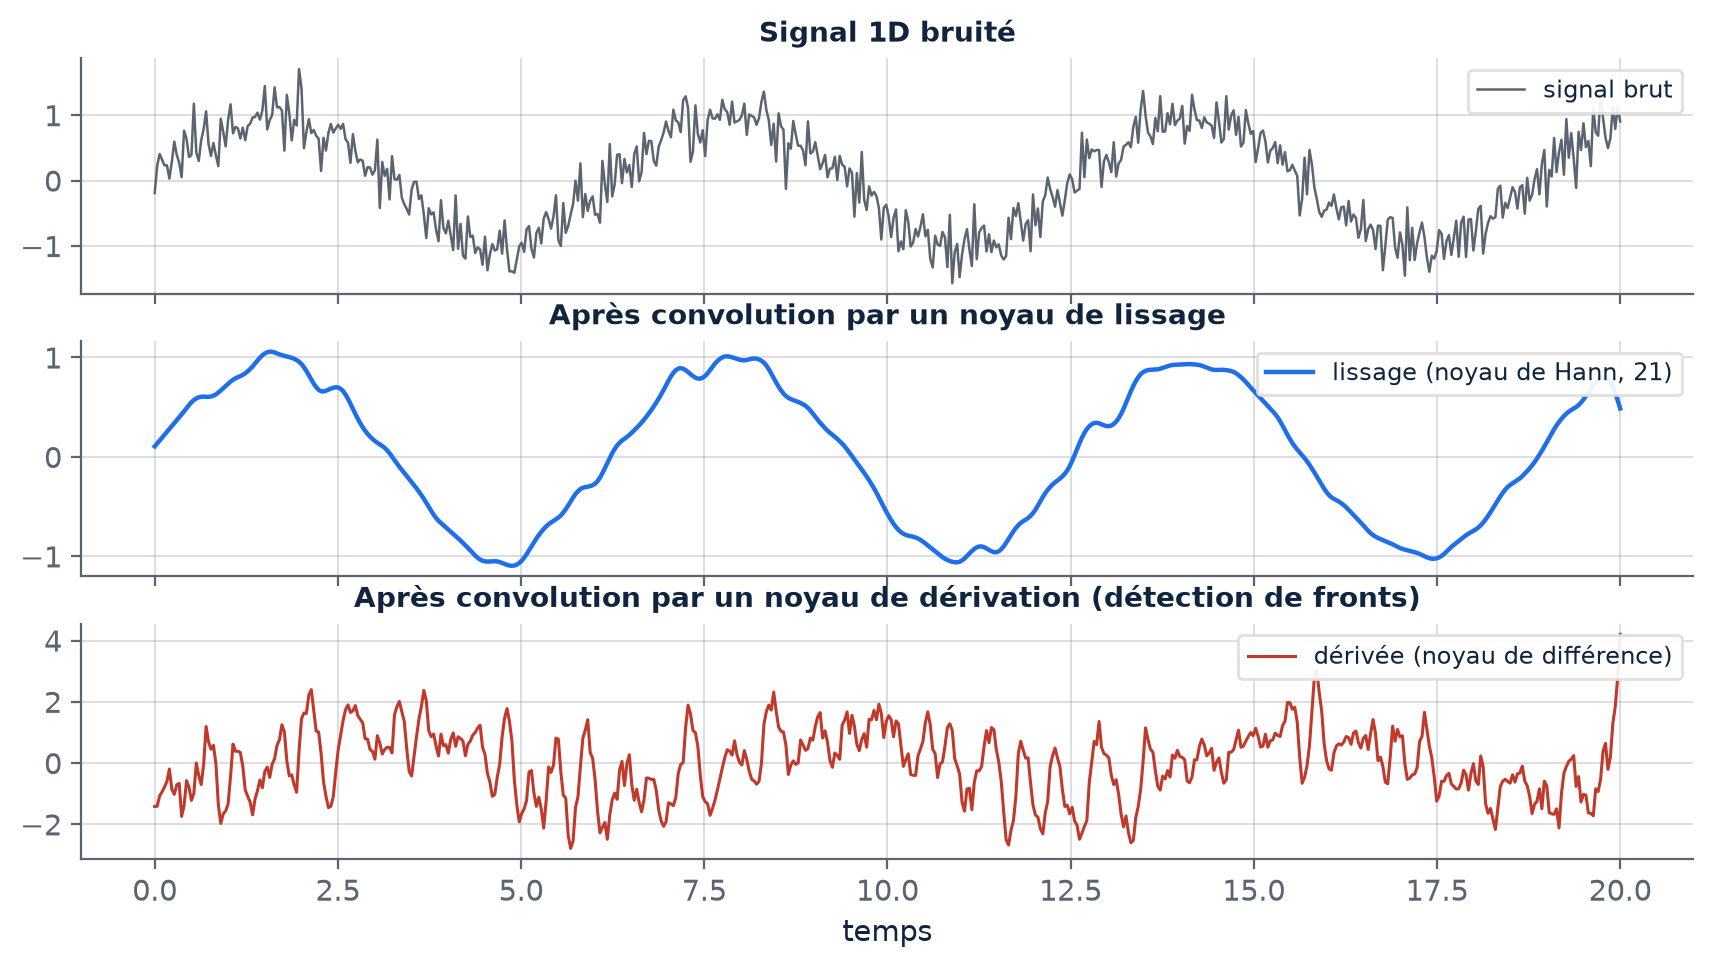
\includegraphics[width=.92\textwidth]{g08_convolution_1d.png}\end{center}\end{frame}

\begin{frame}{1D : le noyau de lissage (Hann, longueur 21)}
\begin{columns}[t]
\begin{column}{0.50\textwidth}
\begin{itemize}
  \item Le noyau de lissage utilisé en 1D est un noyau de \textbf{Hann},
  fenêtre douce de longueur $K = 21$.
  \item Ses coefficients valent
  \[
  w_n = \tfrac{1}{2}\left(1 - \cos\frac{2\pi n}{K-1}\right),
  \quad n = 0,\dots,K-1
  \]
  \item Ils montent de $0$ au centre, puis redescendent symétriquement.
  \item Effet : moyenne locale \textbf{progressive}, sans cassure aux bords
  de la fenêtre --- contrairement à une moyenne glissante uniforme.
\end{itemize}
\end{column}
\begin{column}{0.46\textwidth}
\begin{ebox}[Choisir la largeur du noyau]
Plus $K$ est grand, plus le lissage est fort :
\begin{itemize}
  \item $K$ petit ($\approx 5$) : on gomme le bruit de haute fréquence ;
  \item $K$ grand ($21$) : on ne garde que la tendance lente du signal.
\end{itemize}
\end{ebox}
\begin{wbox}[Compromis]
Un lissage trop fort fait disparaître les accidents que l'on cherche à
détecter : un pic de tachycardie peut être aplati.
\end{wbox}
\end{column}
\end{columns}
\end{frame}

\begin{frame}{1D : le noyau de dérivation (longueur 11)}
\begin{columns}[t]
\begin{column}{0.52\textwidth}
\begin{itemize}
  \item Le noyau de dérivation est un vecteur \textbf{antisymétrique} de
  longueur $K = 11$ : la première moitié est négative, la seconde positive.
  \item Convoluer par ce noyau revient à calculer une \textbf{pente locale},
  lissée sur $11$ points.
  \item Là où le signal est plat, la sortie est nulle ; là où le signal
  change, la sortie est forte.
  \item C'est l'équivalent 1D de Sobel : détecter les \textbf{transitions}.
\end{itemize}
\begin{kbox}[Chaîne classique en 1D]
Lisser (Hann, $K = 21$) \emph{puis} dériver ($K = 11$). Le lissage enlève
le bruit, la dérivation révèle les fronts : pics d'un ECG, sauts de trafic.
\end{kbox}
\end{column}
\begin{column}{0.44\textwidth}
\begin{ebox}[Un front dans un signal]
Signal plat à $0$, puis saut à $100$.
\begin{itemize}
  \item Sortie du noyau de dérivation : nulle avant le saut, fortement
  positive \emph{au} saut, nulle après.
  \item La sortie ne dit pas « il y a $100$ », mais « quelque chose a changé
  ici ».
\end{itemize}
\end{ebox}
\begin{wbox}[Aucune dérivée n'est gratuite]
Dériver amplifie le bruit de haute fréquence ; d'où l'usage systématique
d'un lissage \emph{avant} la dérivation.
\end{wbox}
\end{column}
\end{columns}
\end{frame}

\begin{frame}{1D : la taille de sortie suit la même formule}
\begin{columns}[t]
\begin{column}{0.50\textwidth}
\begin{kbox}[Taille de sortie en 1D (mode valide)]
\[
N_{\text{out}} = N - K + 1
\]
\[
\begin{aligned}
N &= \text{longueur du signal d'entrée},\\
K &= \text{longueur du noyau}.
\end{aligned}
\]
\end{kbox}
\begin{itemize}
  \item Le noyau doit être \textbf{entièrement contenu} dans le signal :
  chaque position utile consomme $K$ points.
  \item C'est la version 1D de la formule $N_{\text{out}} = N - K + 1$ vue
  en 2D sur chaque dimension.
\end{itemize}
\end{column}
\begin{column}{0.46\textwidth}
\begin{ebox}[Application numérique]
Signal de $N = 600$ points et noyau de Hann $K = 21$ :
\[
N_{\text{out}} = 600 - 21 + 1 = 580 \text{ points}
\]
\end{ebox}
\begin{solbox}[Autre repère]
Noyau de dérivation $K = 11$ sur le même signal :
$N_{\text{out}} = 600 - 11 + 1 = 590$ points.
\end{solbox}
\end{column}
\end{columns}
% [fix] bloc deplace
% [fix] bloc deplace
\end{frame}
\begin{frame}{1D : la taille de sortie suit la même fo… (suite)}
\begin{itemize}
  \item Avec le noyau de dérivation ($K = 11$) sur le même signal :
  \[
  N_{\text{out}} = 600 - 11 + 1 = 590 \text{ points}
  \]
  \item Le signal \textbf{raccourcit} : on perd $K - 1$ points au total, soit
  $10$ points avec Hann.
  \item En empilant les couches, le signal rétrécit à chaque étage si l'on
  reste en mode \emph{valide}.
\end{itemize}
\end{frame}
\begin{frame}{1D : la taille de sortie suit la même fo… (suite)}
\begin{wbox}[En pratique]
En mode \emph{same} (remplissage par des zéros ou symétrique), la sortie
garde la longueur de l'entrée : c'est le réglage le plus courant dans un CNN.
\end{wbox}
\end{frame}

\begin{frame}{Applications de la convolution 1D}
\begin{columns}[t]
\begin{column}{0.31\textwidth}
\begin{ebox}[ECG]
Signal cardiaque échantillonné dans le temps. Les noyaux apprennent à
repérer les complexes QRS ; un lissage retire le bruit de mesure avant
l'analyse.
\end{ebox}
\end{column}
\begin{column}{0.31\textwidth}
\begin{ebox}[Trafic routier]
Débit et vitesse par heure ou par minute. Les motifs recherchés sont des
pics matinaux et des creux de nuit : des formes, comme les motifs d'une image.
\end{ebox}
\end{column}
\begin{column}{0.31\textwidth}
\begin{ebox}[Météo]
Température, vent, pression. Un noyau de dérivation repère une chute brutale
de pression ; un lissage dégage la tendance saisonnière.
\end{ebox}
\end{column}
\end{columns}
\vspace{1mm}
\begin{kbox}[Pourquoi cela compte pour ce cours]
Les mêmes noyaux (lissage, dérivation) réapparaissent en 1D, en 2D et en 3D.
Seule change la forme du vecteur de coefficients. Un CNN se définit donc par
sa \emph{forme de noyau}, pas par une modalité de données particulière.
\end{kbox}
\begin{itemize}
  \item Autres usages : signaux industriels (vibrations), audio représenté en
  spectrogramme, texte traité comme une suite de vecteurs.
\end{itemize}
\end{frame}

\begin{frame}[fragile]{Code : appliquer un noyau de Sobel avec scipy}
\begin{columns}[t]
\begin{column}{0.62\textwidth}
\begin{codebox}[scipy.signal.convolve2d]
\begin{lstlisting}
import numpy as np
from scipy.signal import convolve2d

img = np.load("photo_gris.npy")      # image en niveaux de gris

sobel_x = np.array([[-1., 0., 1.],
                    [-2., 0., 2.],
                    [-1., 0., 1.]])
sobel_y = np.array([[-1., -2., -1.],
                    [ 0.,  0.,  0.],
                    [ 1.,  2.,  1.]])

gx = convolve2d(img, sobel_x, mode="same", boundary="symm")
gy = convolve2d(img, sobel_y, mode="same", boundary="symm")

contours = np.hypot(gx, gy)          # amplitude du gradient
contours = contours / contours.max() # -> [0, 1]
np.save("contours.npy", contours)

print(gx.shape, gy.shape, contours.shape)
print(float(contours.min()), float(contours.max()))
\end{lstlisting}
\end{codebox}
\end{column}
\begin{column}{0.36\textwidth}
\begin{itemize}
  \item \py{mode="same"} : la sortie garde la forme de l'entrée.
  \item \py{boundary="symm"} : les bords sont complétés par symétrie, ce qui
  évite un cadre noir artificiel.
  \item \py{np.hypot(gx, gy)} : norme du gradient, insensible au sens du
  contour.
  \item Normaliser avant affichage : les valeurs sont signées et de grande
  amplitude.
\end{itemize}

\end{column}
\end{columns}
% [fix] bloc deplace
\end{frame}
\begin{frame}{Code : appliquer un noyau de Sobel avec … (suite)}
\begin{wbox}[Piège classique]
\py{convolve2d} retourne \py{"full"} par défaut : la sortie est
$N + K - 1$ points de côté, plus grande que l'image. Mettre
\py{mode="same"} sauf besoin précis.
\end{wbox}
\end{frame}

\begin{frame}{Le coût de calcul d'une couche convolutive}
\begin{columns}[t]
\begin{column}{0.52\textwidth}
\begin{kbox}[Nombre d'opérations par couche]
\[
\text{ops} = K^2 \times C_{\text{in}} \times N_{\text{out}}^2 \times C_{\text{out}}
\]
\[
\begin{aligned}
K &= \text{côté du noyau},\\
C_{\text{in}} &= \text{canaux d'entrée},\\
N_{\text{out}} &= \text{côté de la carte de sortie},\\
C_{\text{out}} &= \text{canaux de sortie}.
\end{aligned}
\]
\end{kbox}
\begin{ebox}[Exemple numérique]
$K = 3$, $C_{\text{in}} = 3$, $N_{\text{out}} = 128$,
$C_{\text{out}} = 64$ :
\[
9 \times 3 \times 128^2 \times 64 = 28\,311\,552
\]
soit environ $2{,}8 \times 10^7$ opérations pour \emph{une seule} couche
sur \emph{une seule} image.
\end{ebox}
\end{column}
\begin{column}{0.46\textwidth}
\begin{itemize}
  \item Chaque terme est un facteur d'échelle : quadrupler $C_{\text{out}}$
  quadruple le coût.
  \item Le noyau $K \times K$ coûte quadratiquement en $K$ : passer de
  $3\times3$ à $7\times7$ multiplie par plus de $5$ le travail.
  \item \textbf{Convolution séparable} : si le noyau s'écrit comme le produit
  d'un vecteur colonne et d'un vecteur ligne, on remplace $K^2$ par $2K$ ---
  c'est exactement le cas du flou gaussien et du Hann 1D.
  \item D'où la préférence des architectures pour de \emph{petits noyaux
  empilés} plutôt qu'un grand noyau.
\end{itemize}

\end{column}
\end{columns}
% [fix] bloc deplace
\end{frame}
\begin{frame}{Le coût de calcul d'une couche convolutive (suite)}
\begin{wbox}[Lien avec le mur du MLP]
Le coût est réel, mais il est \emph{partagé} : les mêmes $K^2$ poids servent
pour \emph{toutes} les positions. C'est le partage de poids qui rend le coût
raisonnable, pas le nombre de poids.
\end{wbox}
\end{frame}

\begin{frame}{Quiz : quatre questions}
\begin{qbox}[Question 1 --- Moyenne et flou]
Un noyau dont tous les coefficients valent $1/9$ : quel est son effet ?
\begin{itemize}
  \item[(a)] Il renforce les contours \quad (b) Il floute l'image
  \quad (c) Il ne change rien
\end{itemize}
\end{qbox}
\begin{qbox}[Question 2 --- Le Laplacien]
Que calcule le noyau du Laplacien
$\begin{smallmatrix}0&1&0\\1&-4&1\\0&1&0\end{smallmatrix}$
(centre $-4$, voisins $1$) ?
\begin{itemize}
  \item[(a)] Une moyenne locale \quad (b) Une variation brusque
  (dérivée seconde) \quad (c) Une rotation de l'image
\end{itemize}
\end{qbox}
\begin{qbox}[Question 3 --- Padding « same »]
Une entrée de $5 \times 5$ avec un noyau $3 \times 3$ et un padding
\emph{same} : quelle est la taille de sortie ?
\begin{itemize}
  \item[(a)] $5 \times 5$ \quad (b) $3 \times 3$ \quad (c) $7 \times 7$
\end{itemize}
\end{qbox}
\begin{qbox}[Question 4 --- Stride 2]
Même entrée $5 \times 5$, noyau $3 \times 3$, mais un pas de $2$ (mode
\emph{valide}) : quelle est la taille de sortie ?

\end{qbox}

% [fix] bloc deplace
% [fix] bloc deplace
\end{frame}
\begin{frame}{Quiz : quatre questions (suite)}
\begin{itemize}
  \item[(a)] $3 \times 3$ \quad (b) $2 \times 2$ \quad (c) $1 \times 1$
\end{itemize}
\end{frame}
\begin{frame}{Quiz : quatre questions (suite)}
\begin{solbox}[Réponses]
\textbf{1.} (b) : c'est le flou moyenneur, un passe-bas qui conserve la
luminosité moyenne. \quad
\textbf{2.} (b) : la somme des coefficients est $0$ ; le noyau est nul sur
une zone uniforme et fort sur les variations. \quad
\textbf{3.} (a) : le padding \emph{same} garde la taille, soit $5 \to 5$. \quad
\textbf{4.} (b) : $5 \to 2$ avec un pas de $2$.
\end{solbox}
\end{frame}

\begin{frame}{Quiz : convolution ou corrélation ?}
\begin{columns}[t]
\begin{column}{0.50\textwidth}
\begin{qbox}[Question 5 --- Convolution ou corrélation ?]
En traitement d'image numérique, la « convolution » d'une bibliothèque
comme \py{scipy.signal.convolve2d} et la corrélation croisée diffèrent par
un point. Lequel ?
\begin{itemize}
  \item[(a)] Par le signe du résultat
  \item[(b)] Par le \textbf{retournement} du noyau (rotation de $180^\circ$)
  \item[(c)] Par le pas de balayage
\end{itemize}
\end{qbox}
\begin{solbox}[Réponse]
\textbf{5.} (b) : la convolution \emph{retourne} le noyau ; la corrélation
ne le retourne pas.
\end{solbox}
\end{column}
\begin{column}{0.48\textwidth}
\begin{ebox}[Le noyau, retourné]
\[
K = \begin{smallmatrix}1&2&3\\4&5&6\\7&8&9\end{smallmatrix}
\quad \longrightarrow \quad
K^{\text{retourné}} = \begin{smallmatrix}9&8&7\\6&5&4\\3&2&1\end{smallmatrix}
\]
\end{ebox}
\begin{kbox}[Pourquoi cela n'a pas d'importance en CNN]
Un noyau appris peut toujours compenser le retournement : apprendre
$K$ ou apprendre son image retournée donne exactement les mêmes capacités.
Les bibliothèques d'apprentissage profond utilisent en réalité une
\textbf{corrélation croisée} tout en l'appelant « convolution ».
\end{kbox}

\end{column}
\end{columns}
% [fix] bloc deplace
\end{frame}
\begin{frame}{Quiz : convolution ou corrélation ? (suite)}
\begin{wbox}[Ce qu'il faut retenir]
Pour tout noyau \textbf{symétrique} (flou gaussien, Laplacien, Sobel), la
convolution et la corrélation donnent le \emph{même} résultat.
\end{wbox}
\end{frame}

\begin{frame}{À retenir}
\begin{kbox}[Les cinq points du chapitre]
\begin{enumerate}
  \item La convolution est une \textbf{moyenne pondérée locale} : on fait
  glisser un noyau et on somme les produits point par point.
  \item Le \textbf{noyau} est le seul paramètre de l'opération : sa matrice
  détermine tout l'effet (flou, netteté, contours, relief).
  \item La \textbf{taille de sortie} se calcule par
  $N_{\text{out}} = \lfloor (N + 2p - K)/s \rfloor + 1$, où $p$ est le
  padding et $s$ le pas.
  \item La \textbf{somme des coefficients} résume le comportement : $1$
  conserve l'image, $0$ supprime les zones uniformes.
  \item En 1D comme en 2D, le principe est identique : \textbf{lissage} puis
  \textbf{dérivation} pour révéler les transitions.
\end{enumerate}
\end{kbox}
\vspace{1mm}
\begin{columns}[t]
\begin{column}{0.48\textwidth}
\begin{ebox}[Ce que vous devez savoir faire]

\end{ebox}
\end{column}
\begin{column}{0.48\textwidth}

\end{column}
\end{columns}
% [fix] bloc deplace
% [fix] bloc deplace
\end{frame}
\begin{frame}{À retenir (suite)}
\begin{itemize}
  \item Lire un noyau et prédire son effet.
  \item Calculer une taille de sortie (padding, pas, noyau).
  \item Appliquer un noyau 2D avec \py{scipy.signal.convolve2d}.
\end{itemize}
\end{frame}
\begin{frame}{À retenir (suite)}
\begin{wbox}[Le fil rouge]
Un CNN apprend les coefficients que les ingénieurs écrivaient à la main.
\textbf{La structure est la même ; seul le noyau devient appris.}
\end{wbox}
\end{frame}

\begin{frame}{Travaux pratiques du chapitre}
\begin{columns}[t]
\begin{column}{0.48\textwidth}
\begin{abox}[TP1 --- Noyaux de convolution]
\file{notebooks/TP1_noyaux_convolution.ipynb}
\begin{itemize}
  \item Écrire les noyaux classiques en \py{numpy} (moyenneur, gaussien,
  Sobel, Laplacien).
  \item Les appliquer avec \py{scipy.signal.convolve2d}.
  \item Comparer les effets sur une image synthétique et sur une photo.
  \item Vérifier les tailles de sortie pour \py{mode="full"},
  \py{"same"} et \py{"valid"}.
\end{itemize}
\end{abox}
\end{column}
\begin{column}{0.48\textwidth}
\begin{abox}[TP2 --- Padding, pas, pooling]
\file{notebooks/TP2_padding_stride_pooling.ipynb}
\begin{itemize}
  \item Padding \emph{same} et \emph{valide} sur des tenseurs jouets.
  \item Pas de $1$, $2$, $3$ : mesurer le rétrécissement de la carte de
  sortie.
  \item Max-pooling et moyenne : effet sur la taille et sur les valeurs.
  \item Vérifier chaque résultat à la main \emph{puis} à l'écran.
\end{itemize}
\end{abox}
\end{column}
\end{columns}
\vspace{1mm}

% [fix] bloc deplace
\end{frame}
\begin{frame}{Travaux pratiques du chapitre (suite)}
\begin{kbox}[Objectif des deux séances]
À la fin, vous devez pouvoir dire, devant une carte de sortie quelconque,
comment elle a été obtenue : \textbf{quel noyau, quel padding, quel pas,
quel pooling}.
\end{kbox}
\end{frame}
